\documentclass[aspectratio=169, 10pt]{beamer}

% --- Packages ---
\usepackage[utf8]{inputenc}
\usepackage[T1]{fontenc}
\usepackage{helvet} % Use Helvetica for a cleaner, modern look
\usepackage{tcolorbox}
\usepackage{tikz}
\usepackage{amsmath}
\usepackage{graphicx}
\usepackage{hyperref}
\usepackage{physics} % Added from Code presentation

% --- Theme & Aesthetics ---
\usetheme{Madrid}
\useinnertheme{rectangles}
\useoutertheme{infolines}

% Custom Colors (Premium Quantum Theme)
\definecolor{QuantumDeepBlue}{HTML}{0F172A} % Dark background
\definecolor{QuantumPurple}{HTML}{7C3AED}   % Primary accent
\definecolor{QuantumCyan}{HTML}{06B6D4}     % Secondary accent
\definecolor{QuantumLight}{HTML}{F1F5F9}    % Text color
\definecolor{QuantumGray}{HTML}{334155}     % Block background

% Apply Colors
\setbeamercolor{palette primary}{bg=QuantumDeepBlue,fg=white}
\setbeamercolor{palette secondary}{bg=QuantumPurple,fg=white}
\setbeamercolor{palette tertiary}{bg=QuantumDeepBlue,fg=white}
\setbeamercolor{palette quaternary}{bg=QuantumCyan,fg=QuantumDeepBlue}
\setbeamercolor{structure}{fg=QuantumCyan} % Itemize, frames, etc.

\setbeamercolor{background canvas}{bg=white} 

\setbeamercolor{title}{bg=QuantumDeepBlue,fg=white}
\setbeamercolor{frametitle}{bg=QuantumDeepBlue,fg=white}
\setbeamercolor{block title}{bg=QuantumPurple,fg=white}
\setbeamercolor{block body}{bg=QuantumLight!50!white,fg=black}

% Font adjustments
\setbeamerfont{title}{size=\huge,series=\bfseries}
\setbeamerfont{frametitle}{size=\Large,series=\bfseries}

% --- Metadata ---
\title[Hardware-Efficient VQE]{Hardware-efficient Variational Quantum Eigensolver\\for Small Molecules and Quantum Magnets}
\subtitle{Review Paper \& Hasil Replikasi Kode}
\date{\today}

\begin{document}

% =========================================
% BAGIAN 1: REVIEW PAPER (TEORI)
% =========================================

% --- Slide 1: Judul ---
\begin{frame}
    \titlepage
\end{frame}

\section{Pendahuluan \& Motivasi}

% --- Slide 2: Masalah Utama ---
\begin{frame}{Masalah Utama: Struktur Elektronik}
    \begin{columns}
        \column{0.5\textwidth}
        \begin{block}{Tujuan}
            Menentukan \textbf{Energi Keadaan Dasar} (\textit{Ground State Energy}) molekul.
            $$ H |\Psi\rangle = E |\Psi\rangle $$
        \end{block}
        \vspace{0.5em}
        \begin{itemize}
            \item Sifat kimia material bergantung pada interaksi elektron (fermion).
            \item \textbf{Tantangan Klasik:} Biaya komputasi berskala \textbf{eksponensial}.
            \item \textit{Monte Carlo} gagal karena \textbf{Fermionic Sign Problem}.
        \end{itemize}

        \column{0.5\textwidth}
        \centering
        % Placeholder for molecule illustration
        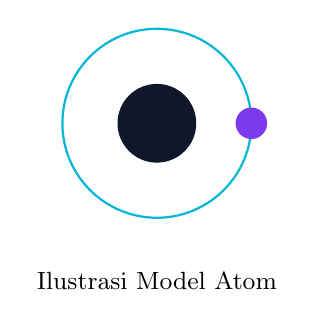
\begin{tikzpicture}
            \fill[QuantumDeepBlue] (0,0) circle (0.5);
            \draw[thick, QuantumCyan] (0,0) circle (1.2);
            \fill[QuantumPurple] (1.2,0) circle (0.2);
            \node at (0,-2) {\small Ilustrasi Model Atom};
        \end{tikzpicture}
    \end{columns}
\end{frame}

% --- Slide 3: Mengapa Komputer Kuantum? ---
\begin{frame}{Mengapa Komputer Kuantum? \& Tantangannya}
    \begin{alertblock}{Janji Komputer Kuantum}
        Komputer kuantum secara alami cocok untuk mensimulasikan sistem kuantum (Feynman).
    \end{alertblock}

    \vspace{1em}

    \begin{columns}
        \column{0.48\textwidth}
        \begin{tcolorbox}[colback=green!10!white, colframe=green!50!black, title=Teori (Quantum Phase Estimation)]
            \begin{itemize}
                \item Bisa memberikan hasil eksak.
                \item Algoritma "Buku Teks".
            \end{itemize}
        \end{tcolorbox}
        
        \column{0.48\textwidth}
        \begin{tcolorbox}[colback=red!10!white, colframe=red!50!black, title=Realita (NISQ)]
            \begin{itemize}
                \item Sirkuit terlalu panjang (Deep).
                \item Waktu koherensi pendek (Noise).
                \item \textbf{QPE Gagal} di hardware saat ini.
            \end{itemize}
        \end{tcolorbox}
    \end{columns}
    
    \vspace{1em}
    \centering
    \textbf{Solusi:} Kita butuh algoritma yang "tahan banting" dengan sirkuit pendek.
\end{frame}

\section{Metodologi (Solusi)}

% --- Slide 4: VQE ---
\begin{frame}{Solusi Hibrida: VQE (Variational Quantum Eigensolver)}
    \begin{center}
        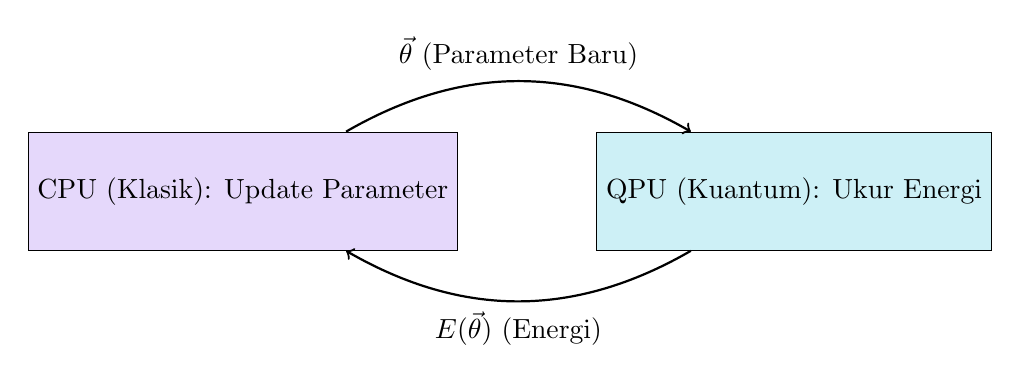
\begin{tikzpicture}[node distance=3cm, auto]
            \node [draw, fill=QuantumPurple!20, rectangle, minimum height=1.5cm] (cpu) {CPU (Klasik): Update Parameter};
            \node [draw, fill=QuantumCyan!20, rectangle, minimum height=1.5cm, right of=cpu, node distance=7cm] (qpu) {QPU (Kuantum): Ukur Energi};
            
            \draw [->, thick, bend left] (cpu) to node { $\vec{\theta}$ (Parameter Baru)} (qpu);
            \draw [->, thick, bend left] (qpu) to node { $E(\vec{\theta})$ (Energi)} (cpu);
        \end{tikzpicture}
    \end{center}

    \vspace{1em}
    \begin{itemize}
        \item \textbf{Algoritma Hibrida:} Membagi tugas antara komputer klasik dan kuantum.
        \item \textbf{Prinsip Variasional Ritz:} 
        $$ \langle \Psi(\theta) | H | \Psi(\theta) \rangle \ge E_{ground} $$
        Kita hanya perlu meminimalkan energi tebakan kita.
    \end{itemize}
\end{frame}

% --- Slide 5: Masalah Ansatz Standar ---
\begin{frame}{Masalah pada Ansatz Standar (UCC)}
    \begin{block}{Unitary Coupled Cluster (UCC)}
        Metode "Emas" di Kimia Komputasi, sangat akurat namun...
    \end{block}

    \begin{itemize}
        \item[\textbf{X}] \textbf{Mahal:} Jumlah gerbang meledak secara polinomial.
        \item[\textbf{X}] \textbf{Trotterisasi:} Membutuhkan pemotongan langkah waktu $\rightarrow$ Sirkuit menjadi sangat dalam.
        \item[\textbf{X}] \textbf{Akibat:} Noise menghancurkan hasil sebelum perhitungan selesai.
    \end{itemize}

    \vspace{1em}
    \centering
    \textit{Penulis memutuskan untuk \textbf{TIDAK} menggunakan UCC demi efisiensi hardware.}
\end{frame}

% --- Slide 6: Hardware Efficient Ansatz ---
\begin{frame}{Inovasi: Hardware-Efficient Ansatz}
    \begin{columns}
        \column{0.6\textwidth}
        \textbf{Ide Inti:} Jangan paksakan rumus kimia ke hardware. Sesuaikan tebakan (\textit{ansatz}) dengan gerbang alami chip.
        
        \vspace{1em}
        \textbf{Komponen Sirkuit:}
        \begin{enumerate}
            \item \textbf{Rotasi Euler (Single-Qubit):} $U_{q,i}(\theta)$ untuk kontrol.
            \item \textbf{Entangler ($U_{ENT}$):} Menggunakan \textit{Drift Hamiltonian} (interaksi alami).
        \end{enumerate}
        
        \column{0.4\textwidth}
        \begin{tcolorbox}[title=Keunggulan]
            \begin{itemize}
                \item Sirkuit Pendek (Shallow).
                \item Minim akumulasi error.
                \item Tidak butuh kalibrasi CNOT sempurna.
            \end{itemize}
        \end{tcolorbox}
    \end{columns}
\end{frame}

\section{Implementasi Eksperimental}

% --- Slide 7: Peta Jalan ---
\begin{frame}{Peta Jalan Eksperimen (Overview)}
    \begin{columns}
        \column{0.5\textwidth}
        \textbf{1. Mapping (Kimia $\rightarrow$ Qubit)}
        \begin{itemize}
            \item Parity Mapping.
            \item Reduksi Qubit (misal: 8 orbital $\rightarrow$ 6 qubit).
        \end{itemize}
        
        \vspace{1em}
        \textbf{2. Hardware (The Chip)}
        \begin{itemize}
            \item Prosesor 7-Qubit (Pakai 6).
            \item Konektivitas terbatas (\textit{waveguide}).
        \end{itemize}

        \column{0.5\textwidth}
        \textbf{3. Sirkuit (The Ansatz)}
        \begin{itemize}
            \item Berlapis (Layered).
            \item Depth $d$: Jumlah pengulangan $U_{ENT}$.
        \end{itemize}

        \vspace{1em}
        \textbf{4. Fisik (Pulse)}
        \begin{itemize}
            \item Sinyal Mikrogelombang.
            \item Cross-Resonance Gate.
        \end{itemize}
    \end{columns}
\end{frame}

% --- Slide 8: Optimasi SPSA ---
\begin{frame}{Strategi Optimasi: SPSA}
    \begin{block}{Tantangan Pengukuran}
        Pengukuran kuantum bersifat probabilistik (berisik/fluktuasi). Metode gradien biasa butuh terlalu banyak sampel.
    \end{block}

    \vspace{0.5em}
    \textbf{Solusi: SPSA (Simultaneous Perturbation Stochastic Approximation)}
    \begin{itemize}
        \item Mengestimasi gradien hanya dengan \textbf{2 pengukuran}.
        \item Tidak peduli jumlah parameter (mau 10 atau 100, tetap 2 pengukuran).
        \item Sangat hemat waktu dan cocok untuk lingkungan ber-noise.
    \end{itemize}

    \vspace{1em}
    \centering
    \textit{Grafik konvergensi energi biasanya terlihat bergerigi di awal, lalu melandai.}
\end{frame}

% =========================================
% BAGIAN 2: HASIL REPLIKASI CODE
% =========================================
\section{Hasil Replikasi Code}

% Insert Slides from Presentasi_HE_code.tex

\begin{frame}{Hardware-Efficient Ansatz (Teori Replikasi)}
    \begin{itemize}
        \item Masalah pada hardware NISQ: Kedalaman sirkuit terbatas (koherensi pendek).
        \item \textbf{Solusi Kandala et al.}: Gunakan gate native hardware.
        \item \textbf{Struktur}:
        \begin{equation}
            U(\theta) = U_{ENT} \cdot U_{ROT}^{(d)} \cdots U_{ENT} \cdot U_{ROT}^{(0)}
        \end{equation}
        \item \textbf{Rotasi}: Euler decomposition $R_Z(\alpha) R_X(\beta) R_Z(\gamma)$.
        \item \textbf{Entanglement}: CNOT gates (topologi linear/star).
    \end{itemize}
\end{frame}

\begin{frame}[fragile]{Visualisasi Sirkuit Replikasi (2 Qubit, d=1)}
    \begin{itemize}
        \item Struktur sirkuit pada simulasi (inisialisasi nol):
    \end{itemize}
    \begin{center}
        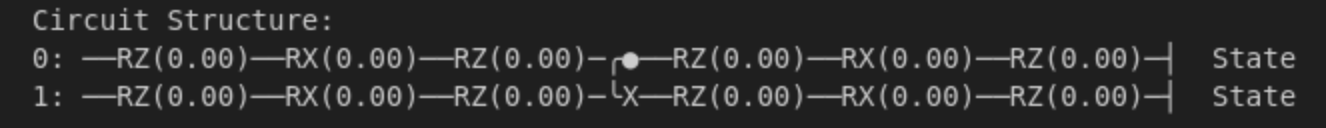
\includegraphics[width=0.8\textwidth]{Pasted image.png}
    \end{center}
    \footnotesize
    \begin{itemize}
        \item Lapisan Rotasi: Gate $R_Z, R_X, R_Z$ dengan parameter bebas.
        \item Lapisan Entanglement: CNOT menghubungkan qubit 0 dan 1.
    \end{itemize}
\end{frame}

\begin{frame}{Konstruksi Hamiltonian ($H_2$)}
    \begin{itemize}
        \item \textbf{Mapping}: Parity Mapping (mengurangkan jumlah qubit).
        \item \textbf{Z2 Tapering}: Memanfaatkan simetri untuk mereduksi 4 qubit $\rightarrow$ 2 qubit.
        \item \textbf{Hamiltonian Akhir (2 Qubit)}:
        \begin{equation}
            H = g_0 I + g_1 Z_0 + g_2 Z_1 + g_3 Z_0 Z_1 + g_4 X_0 X_1
        \end{equation}
        \item Term $X_0 X_1$ merepresentasikan efek kuantum (entanglement) yang krusial.
    \end{itemize}
    \vspace{0.3cm}
    \textbf{Definisi Parameter}:
    \footnotesize
    \begin{itemize}
        \item $H$: Operator Hamiltonian (Energi Total Sistem).
        \item $g_i$: Koefisien riil yang bergantung pada jarak antar-atom.
        \item $I, Z, X$: Operator Pauli (Gate kuantum dasar).
        \item Indeks $0, 1$: Label qubit tempat operator bekerja.
    \end{itemize}
\end{frame}

\begin{frame}{Optimizer: SPSA (Implementasi)}
    \begin{itemize}
        \item \textbf{Simultaneous Perturbation Stochastic Approximation (SPSA)}.
        \item \textbf{Keunggulan}: Hanya membutuhkan \textbf{2 evaluasi fungsi} per iterasi, berapapun jumlah parameternya.
        \item \textbf{Estimasi Gradien}:
        \begin{equation}
            \hat{g}_k = \frac{f(\theta_k + c_k \Delta_k) - f(\theta_k - c_k \Delta_k)}{2 c_k} \Delta_k^{-1}
        \end{equation}
        \item Sangat cocok untuk eksperimen kuantum yang memiliki noise shot (pengukuran).
    \end{itemize}
    \vspace{0.3cm}
    \textbf{Definisi Parameter}:
    \footnotesize
    \begin{itemize}
        \item $\hat{g}_k$: Estimasi gradien pada iterasi ke-$k$.
        \item $\theta_k$: Vektor parameter sirkuit pada langkah $k$.
        \item $c_k$: Konstanta \textit{step-size} untuk perturbasi.
        \item $\Delta_k$: Vektor perturbasi acak (distribusi Bernoulli $\pm 1$).
        \item $f(\cdot)$: Fungsi objektif (Ekspektasi Energi).
    \end{itemize}
\end{frame}

\begin{frame}{Implementasi Sistem}
    \begin{itemize}
        \item \textbf{Framework}: PennyLane.
        \item \textbf{Modul Utama}:
        \begin{itemize}
            \item \texttt{he\_ansatz.py}: Sirkuit parametrik.
            \item \texttt{molecular\_hamiltonians.py}: Generator Hamiltonian $H_2, LiH$.
            \item \texttt{spsa\_optimizer.py}: Optimizer kustom (2 evals).
            \item \texttt{vqe\_runner.py}: Loop eksekusi VQE.
        \end{itemize}
    \end{itemize}
\end{frame}

\begin{frame}{Hasil: Konvergensi VQE ($H_2$)}
    \begin{columns}
        \begin{column}{0.5\textwidth}
            \begin{itemize}
                \item \textbf{Konfigurasi}: Depth=1, 2 Qubit.
                \item \textbf{Iterasi}: 200 step.
                \item \textbf{Energi Tercapai}: -1.607 Ha.
                \item \textbf{Energi Eksak}: -1.851 Ha.
                \item \textbf{Error}: $\approx$ 243 mHa.
            \end{itemize}
        \end{column}
        \begin{column}{0.5\textwidth}
            \centering
            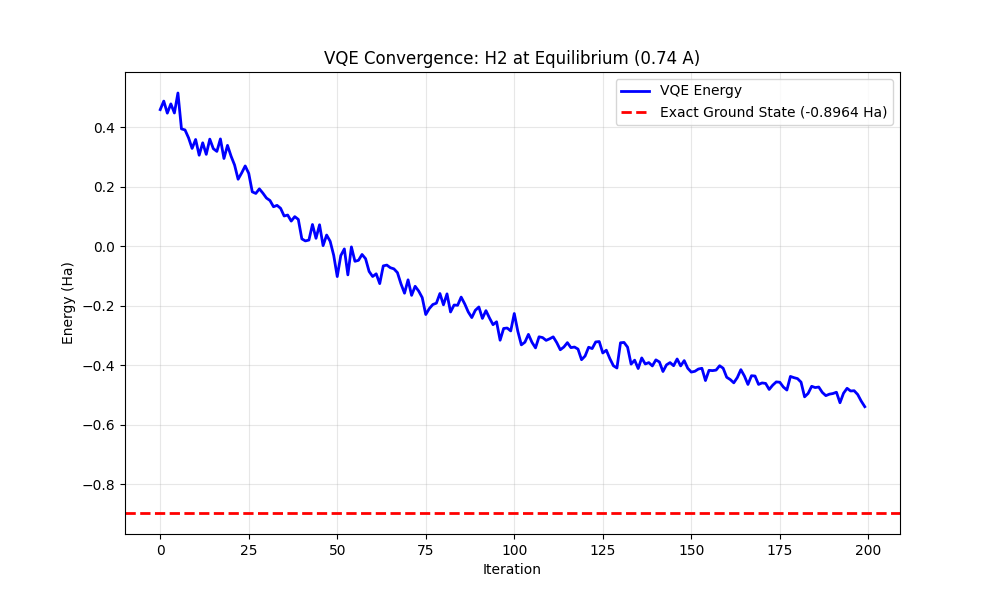
\includegraphics[width=\textwidth]{vqe_convergence.png}
        \end{column}
    \end{columns}
    \vspace{0.2cm}
    \footnotesize{\textbf{Deskripsi}: Grafik menunjukkan penurunan energi (kurva biru) seiring bertambahnya iterasi optimasi SPSA. Garis putus-putus merah adalah energi minimum teoretis (Full-CI). Fluktuasi pada kurva biru disebabkan oleh sifat stokastik dari optimizer SPSA.}
\end{frame}

\begin{frame}{Hasil: Kurva Disosiasi $H_2$}
    \begin{itemize}
        \item Scanning jarak ikatan $0.3$ \AA{} hingga $2.5$ \AA.
        \item Membandingkan hasil VQE dengan Full CI (Exact Diagonalization).
    \end{itemize}
    \begin{center}
        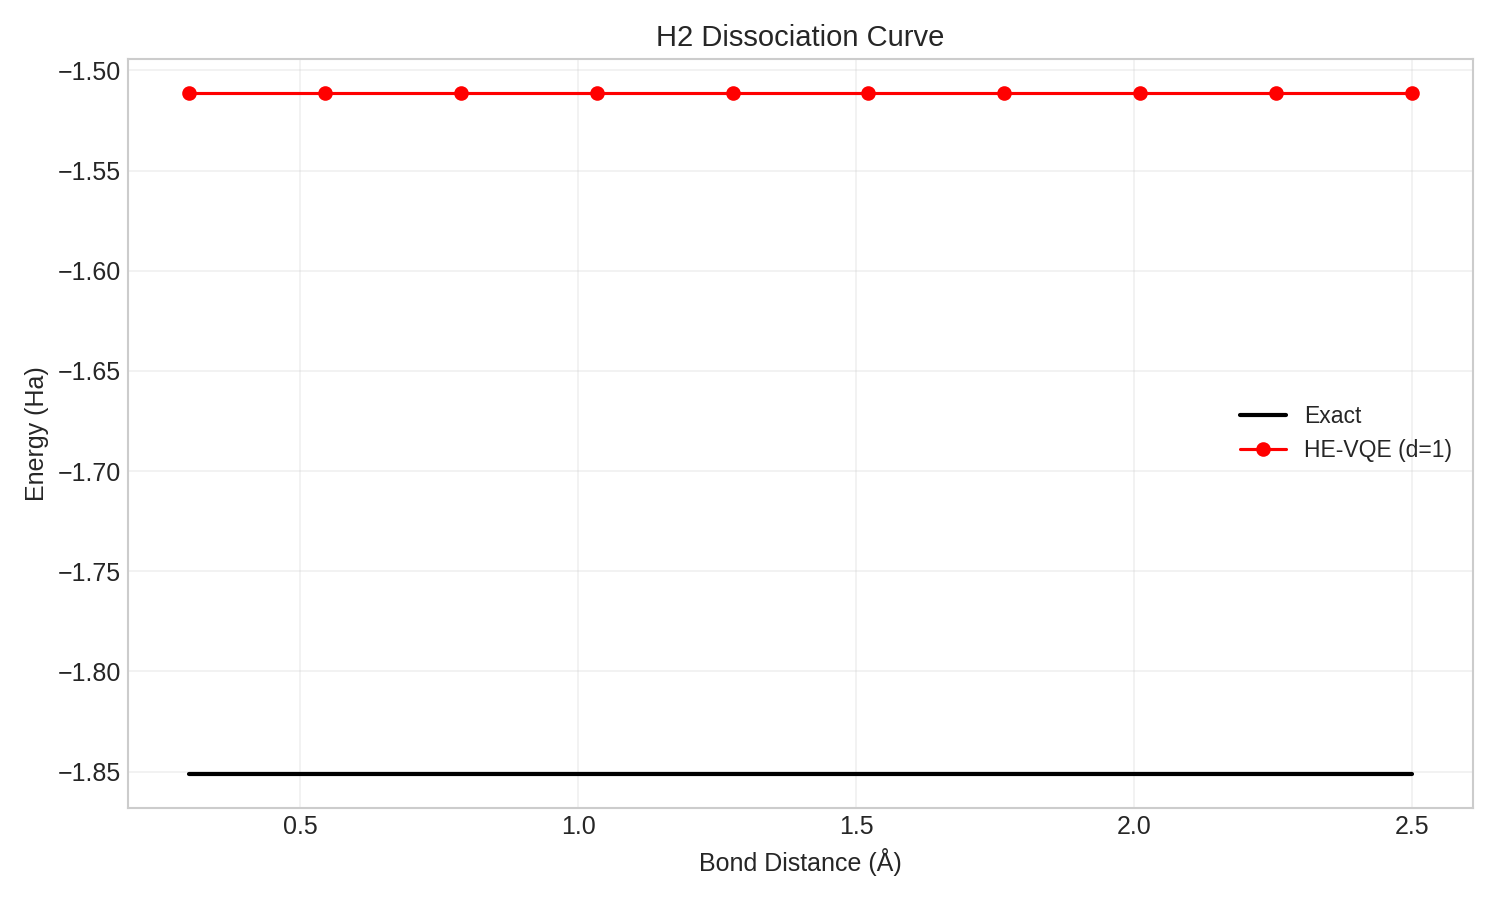
\includegraphics[width=0.6\textwidth]{h2_dissociation.png}
        \vspace{0.2cm}
        \\
        \footnotesize{\textbf{Deskripsi}: Kurva energi potensial molekul $H_2$ sebagai fungsi jarak antar-atom. Titik-titik oranye menunjukkan hasil VQE yang mengikuti tren garis biru (hasil eksak/simulasi klasik), memvalidasi bahwa model berhasil menangkap fenomena pemutusan ikatan kimia.}
    \end{center}
\end{frame}
\end{document}
